\documentclass{beamer}

\pdfmapfile{+sansmathaccent.map}


\mode<presentation>
{
  \usetheme{Warsaw} % or try Darmstadt, Madrid, Warsaw, Rochester, CambridgeUS, ...
  \usecolortheme{seahorse} % or try seahorse, beaver, crane, wolverine, ...
  \usefonttheme{serif}  % or try serif, structurebold, ...
  \setbeamertemplate{navigation symbols}{}
  \setbeamertemplate{caption}[numbered]
} 


%%%%%%%%%%%%%%%%%%%%%%%%%%%%
% itemize settings

\definecolor{mypink}{RGB}{255, 30, 80}
\definecolor{mydarkblue}{RGB}{60, 160, 255}
\definecolor{myblackblue}{RGB}{40, 40, 120}
\definecolor{myblue}{RGB}{240, 240, 255}
\definecolor{mygreen}{RGB}{0, 200, 0}
\definecolor{mygreen2}{RGB}{205, 255, 200}
\definecolor{mygray}{gray}{0.8}
% \definecolor{mydarkgray}{gray}{0.4}
\definecolor{mydarkgray}{RGB}{80, 80, 160}

\setbeamertemplate{itemize items}[default]

\setbeamertemplate{itemize item}{\color{myblackblue}$\blacksquare$}
\setbeamertemplate{itemize subitem}{\color{mydarkblue}$\blacktriangleright$}
\setbeamertemplate{itemize subsubitem}{\color{mygray}$\blacksquare$}

\setbeamercolor{palette quaternary}{fg=white,bg=mydarkgray}
\setbeamercolor{titlelike}{parent=palette quaternary}

\setbeamercolor{palette quaternary2}{fg=black,bg=myblue}
\setbeamercolor{frametitle}{parent=palette quaternary2}

\setbeamerfont{frametitle}{size=\Large,series=\scshape}
\setbeamerfont{framesubtitle}{size=\normalsize,series=\upshape}





%%%%%%%%%%%%%%%%%%%%%%%%%%%%
% block settings

\setbeamercolor{block title}{bg=red!30,fg=black}

\setbeamercolor*{block title example}{bg=mygreen!40!white,fg=black}

\setbeamercolor*{block body example}{fg= black, bg= mygreen2}


%%%%%%%%%%%%%%%%%%%%%%%%%%%%
% URL settings
\hypersetup{
    colorlinks=true,
    linkcolor=blue,
    filecolor=blue,      
    urlcolor=blue,
}

%%%%%%%%%%%%%%%%%%%%%%%%%%

\renewcommand{\familydefault}{\rmdefault}

\usepackage{amsmath}
\usepackage{mathtools}

\usepackage{subcaption}

\usepackage{qrcode}

\DeclareMathOperator*{\argmin}{arg\,min}
\newcommand{\bo}[1] {\mathbf{#1}}

\newcommand{\dx}[1] {\dot{\mathbf{#1}}}
\newcommand{\ma}[4] {\begin{bmatrix}
    #1 & #2 \\ #3 & #4
    \end{bmatrix}}
\newcommand{\myvec}[2] {\begin{bmatrix}
    #1 \\ #2
    \end{bmatrix}}
\newcommand{\myvecT}[2] {\begin{bmatrix}
    #1 & #2
    \end{bmatrix}}
    
    

\newcommand{\mydate}{Spring 2022}
\newcommand{\mygit}{\textcolor{blue}{\href{https://github.com/SergeiSa/Control-Theory-Slides-Spring-2022}{github.com/SergeiSa/Control-Theory-Slides-Spring-2022}}}


\newcommand{\bref}[2] {\textcolor{blue}{\href{#1}{#2}}}




%%%%%%%%%%%%%%%%%%%%%%%%%%%%
% code settings

\usepackage{listings}
\usepackage{color}
% \definecolor{mygreen}{rgb}{0,0.6,0}
% \definecolor{mygray}{rgb}{0.5,0.5,0.5}
\definecolor{mymauve}{rgb}{0.58,0,0.82}
\lstset{ 
  backgroundcolor=\color{white},   % choose the background color; you must add \usepackage{color} or \usepackage{xcolor}; should come as last argument
  basicstyle=\footnotesize,        % the size of the fonts that are used for the code
  breakatwhitespace=false,         % sets if automatic breaks should only happen at whitespace
  breaklines=true,                 % sets automatic line breaking
  captionpos=b,                    % sets the caption-position to bottom
  commentstyle=\color{mygreen},    % comment style
  deletekeywords={...},            % if you want to delete keywords from the given language
  escapeinside={\%*}{*)},          % if you want to add LaTeX within your code
  extendedchars=true,              % lets you use non-ASCII characters; for 8-bits encodings only, does not work with UTF-8
  firstnumber=0000,                % start line enumeration with line 0000
  frame=single,	                   % adds a frame around the code
  keepspaces=true,                 % keeps spaces in text, useful for keeping indentation of code (possibly needs columns=flexible)
  keywordstyle=\color{blue},       % keyword style
  language=Octave,                 % the language of the code
  morekeywords={*,...},            % if you want to add more keywords to the set
  numbers=left,                    % where to put the line-numbers; possible values are (none, left, right)
  numbersep=5pt,                   % how far the line-numbers are from the code
  numberstyle=\tiny\color{mygray}, % the style that is used for the line-numbers
  rulecolor=\color{black},         % if not set, the frame-color may be changed on line-breaks within not-black text (e.g. comments (green here))
  showspaces=false,                % show spaces everywhere adding particular underscores; it overrides 'showstringspaces'
  showstringspaces=false,          % underline spaces within strings only
  showtabs=false,                  % show tabs within strings adding particular underscores
  stepnumber=2,                    % the step between two line-numbers. If it's 1, each line will be numbered
  stringstyle=\color{mymauve},     % string literal style
  tabsize=2,	                   % sets default tabsize to 2 spaces
  title=\lstname                   % show the filename of files included with \lstinputlisting; also try caption instead of title
}


%%%%%%%%%%%%%%%%%%%%%%%%%%%%
% URL settings
\hypersetup{
    colorlinks=false,
    linkcolor=blue,
    filecolor=blue,      
    urlcolor=blue,
}

%%%%%%%%%%%%%%%%%%%%%%%%%%

%%%%%%%%%%%%%%%%%%%%%%%%%%%%
% tikz settings

\usepackage{tikz}
\tikzset{every picture/.style={line width=0.75pt}}


\title{Differential equations}
\subtitle{Math and modeling for high school}
\author{by Sergei Savin}
\centering
\date{Fall 2022}



\begin{document}
\maketitle


\begin{frame}{Derivatives and predictions}
	% \framesubtitle{Part 1}
	\begin{flushleft}
		
		Consider a function $y = y(x)$, with a derivative $\frac{d}{dx} y = \dot y$. Assume that $y(0) = 10$ and $\dot y (0) = 1$. Can we find (approximately) what $y(\Delta x)$ is, if $\Delta x$ is very small?
		
		\bigskip
		
		We can reasonably say that $y(\Delta x) \approx y(0) + \dot y (0) \Delta x$.
		
		% TODO: \usepackage{graphicx} required
		\begin{figure}
			\centering
			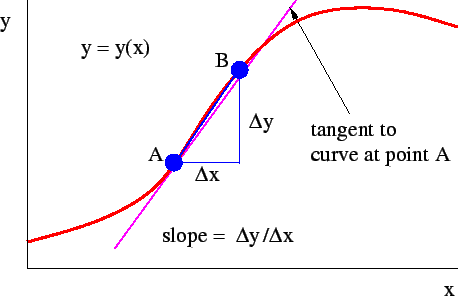
\includegraphics[width=0.7\linewidth]{tangent_to_curve2}
			\label{fig:tangenttocurve2}
		\end{figure}
		
		
	\end{flushleft}
\end{frame}



\begin{frame}{Derivatives and predictions}
	% \framesubtitle{Part 1}
	\begin{flushleft}
		
		More generally:
		
		 $$y(x + \Delta x) \approx y(x) + \dot y (x) \Delta x$$ 
	
		If this approximation is accurate enough, it appears we could draw a graph of a function while knowing only its slopes (derivatives) $\dot y = \dot y (x)$.
		
		
		
	\end{flushleft}
\end{frame}




\begin{frame}{Derivatives and equations}
	% \framesubtitle{Part 1}
	\begin{flushleft}
		
		Consider a ``usual" function $y = y(x)$. For example, $y(x) = x^3 - 1$. We define it by identifying how $y$ depends on $x$. In other words - we explain which $y$ we expect for a given $x$.
		
		\bigskip
		
		But what if instead we identify what rate of change (slope) of the function we expect for a given $x$? Can we define a graph as $\dot y =\dot y(x)$?
		
	\end{flushleft}
\end{frame}



\begin{frame}{Derivatives and equations}
	% \framesubtitle{Part 1}
	\begin{flushleft}
		
		Let us look at an example. Consider a function $\dot y =2x$.
		
		\bigskip
		
		We remember that a derivative of $x^2$ is $2x$. So, is graph $\dot y =2x$ equivalent to $y =x^2$?
		
		\bigskip
		
		Remember that $\frac{d}{dx} (x^2 - 1) = 2x$, and $\frac{d}{dx} (x^2 + 20) = 2x$, and $\frac{d}{dx} (x^2 + 3) = 2x$. 
		
		\begin{block}{Differential equation}
		So, $\dot y =2x$ is not equivalent to any one of those graphs, it actually describes a family of graphs $y =x^2 + c$, $c = const$. We call it \emph{differential equation}.
		\end{block}
		
	\end{flushleft}
\end{frame}




\begin{frame}{Initial conditions}
	% \framesubtitle{Part 1}
	\begin{flushleft}
		
		Given differential equation $\dot y =2x$ and knowing what the function is equal to at a single point (if $x = 0$, then $y = 7$ - as an example) is sufficient to recover the function; not a family of graphs, but one concrete graph.
		
		\bigskip
		
		Let us test it. We know that $y =x^2 + c$, and also that if $x = 0$, then $y = 7$. So, $7 =0^2 + c$, hence $c = 7$. The graph we recovered is:
		
		\begin{equation}
			y =x^2 + 7
		\end{equation}
		
	\end{flushleft}
\end{frame}



\begin{frame}{Initial conditions}
	% \framesubtitle{Part 1}
	\begin{flushleft}
		
		If we know what $y$ is when $x = 0$, this is called \emph{initial conditions}. Knowing a differential equation and initial conditions we can \emph{solve} it - which means we can recover a single graph it represents for those initial conditions.
		
		\bigskip
		
		This makes sense if we think back to our approximation $y(x + \Delta x) \approx y(x) + \dot y (x) \Delta x$. We can use it to continue a graph from a certain point, but not to draw it from scratch. It is very explicit at the point $x = 0$:
		
		$$y(\Delta x) \approx y(0) + \dot y (0) \Delta x$$
		
		If we know $y(0)$ and how to find $\dot y$, we can approximate the whole graph. 
		
	\end{flushleft}
\end{frame}



\begin{frame}{Differential equations}
	% \framesubtitle{Part 1}
	\begin{flushleft}
		
		Some differential equations naturally make sense:
		
		$$\dot y = x$$
		$$\dot y = 4x^3 + 1$$
		$$\dot y = -1$$
		
		But they don't need to be simple. For example, we can write the following differential equation:
		
		$$\dot y = -y$$.
		
		And indeed, if we know what $y$ is when $x = 0$, then we can approximate its solution.
		
	\end{flushleft}
\end{frame}





\begin{frame}{Thank you!}
\centerline{Lecture slides are available via Moodle.}
\bigskip
\centerline{You can help improve these slides at:}
\centerline{\mygit}
\bigskip
\centerline{Check Moodle for additional links, videos, textbook suggestions.}
\bigskip

\centerline{\textcolor{black}{\qrcode[height=1.6in]{https://github.com/SergeiSa/Extra-math-for-high-school}}}

\end{frame}

\end{document}
